% !TEX encoding = UTF-8 Unicode
\documentclass{sig-alternate}
\usepackage{textcomp}
\usepackage{graphics}
\usepackage[utf8]{inputenc}
\usepackage[T1]{fontenc}
\usepackage{listings}

\hyphenation{o-pe-ra-do-res}

\begin{document}

\pagenumbering{arabic}

\title{Algoritmos Genéticos}
\subtitle{Sistemas de Inteligencia Artificial - ITBA}

\numberofauthors{3}

\author{
	\alignauthor{Carlos Sessa}\\
	\alignauthor{Lucas Pizzagalli}\\
	\alignauthor{Nicolás Purita}\\	
}

\date{12 de Junio de 2012}

\maketitle

\section{Introducción}

	Se implementa un motor de algoritmos genéticos para obtener los pesos para la red neuronal construida en el Trabajo Práctico Especial Número 2.
	La red neuronal resuelve la función que se puede observar en la figura \ref{fig:function}.

	\begin{figure}[!ht]
		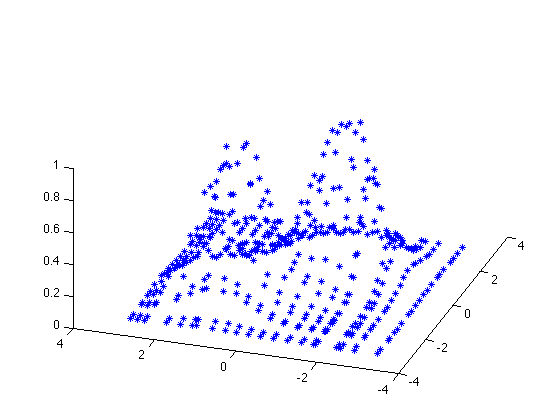
\includegraphics[scale=0.5]{./figures/function.png}
  		\caption{Distribución de puntos dada}
  		\label{fig:function}
	\end{figure}

	En la figura \ref{fig:function} se puede observar que los puntos de la entrada pertenecen al intervalo $[-3.5, 3.5]$ y la salida se encuentra en el intervalo $(0, 1)$.\\
	El algoritmo genético se implementó en \textit{Java} y la red neuronal fue realizada en \textit{Matlab}. Utilizando el \textit{MATLAB Compiler Runtime} se realizan las pruebas pertinentes para verificar el funcionamiento de la red.\\

\section{Desarrollo y Problemas encontrados}
Se han implementado varios operadores genéticos, métodos de selección, condiciones de corte y demás configuraciones que se presentarán en las secciones a continuación.
Con el objetivo de facilitar la configuración se ha creado un archivo de
\textit{properties} en el que se debe detallar como se desea entrenar la red.
Un ejemplo de dicho archivo se puede observar en la lista \ref{code:simple}.

	\subsection{Operadores genéticos}
	\subsubsection{Mutación}
	Las mutaciones se realizan tomando un número aleatorio definido entre $-1.5$ y $1.5$.
	Se han implementado las mutaciones del tipo clásicas y no uniformes.

	\subsubsection{Crossover}
	Se han decidido implementar los siguientes algoritmos de cruzamiento:
	\begin{itemize}
		\item cruce de un punto (clásica)
		\item cruce de dos puntos
		\item cruce anular
		\item cruce uniforme parametrizado
		\item Gene
	\end{itemize}

	\textit{Gene} funciona de manera similar al cruce clásico pero en vez de
	realizar el cruce en base a un \textit{locus} lo hace reemplazando
	capas enteras.

	\subsubsection{Backpropagation}
	Otro operador utilizado es \textit{Backpropagation}.
	El mismo toma como parámetro la cantidad de épocas que debe entrenar la red.

	\subsection{Métodos de selección y reemplazo}
	Para ambos casos se han desarrollado los métodos descriptos a
	continuación, los cuales pueden ser combinados:
	\begin{itemize}
		\item Método de elitismo
		\item Método de torneos
		 \item Método de Boltzman
		 \item Método de selección universal estocástica
	\end{itemize}

	\subsection{Distintas arquitecturas}
	Mediante el archivo de configuración se puede seleccionar la arquitectura que se desea utilizar para realizar las pruebas. Las arquitecturas a elegir son las siguientes:

	\begin{center}
		\begin{enumerate}
			\item $[30\,\,20\,\,10\,\,1]$
			\item $[10\,\,10\,\,1]$
			\item $[10\,\,\,1]$
			\item $[10\,\,10\,\,10\,\,10\,\,1]$
			\item $[40\,\,20\,\,1]$
			\item $[10\,\,10\,\,10\,\,1]$
			\item $[5\,\,10\,\,20\,\,1]$
		\end{enumerate}
	\end{center}

	\subsection{Representación del individuo}
	Con el objetivo de representar al individuo, se ha elegido transformar
	la matriz a un vector de números \textit{doubles} como se muestra en
	la figura \ref{fig:indiv} y de esta forma poder aplicar los operadores
	pertinentes de una forma rápida y sencilla.

	Esta representación no se adapta a la representación de la matriz en
	\textit{MATLAB}, por lo tanto se realiza una transformación del individuo.
	Esta transformación consiste en cambiar el vector de doubles por una
	matriz y viceversa.

	\subsubsection{Fidelidad del individuo}

	\begin{itemize}

		\item \textbf{Completitud}: Es completa ya que se puede representar todo el dominio del problema.

		\item \textbf{Coherencia}: Representa únicamente el dominio del problema, ya que ninguna representación puede pertenecer a un conjunto fuera del dominio.

		\item \textbf{Uniformidad}: Se puede concluir que esta representación es uniforme ya que es imposible representar dos individuos distintos con la misma cadena, en caso que esto sucediera esa representación sería exactamente la misma que la otra.	

		\item \textbf{Sencillez}: Convertir matriz de pesos a un vector de doubles es una operación simple.

		\item \textbf{Localidad}: Es local dada que un cambio en un elemento
		del vector genera un cambio en el peso de la conexión que representa.

	\end{itemize}
	
\section{Resultados y Conclusiones}
	Los resultados se presentadan en dos secciones distintas.
	En la primera no se utilizará el operador backpropagation y la segunda sí. \\

	Con el fin de obtener resultados comparables entre sí se define un
	contexto base para todas las pruebas de cada sección.
	Luego en cada prueba se reemplaza el caso base con lo que se desea.
	Debe tenerse en cuenta que el hecho de prefijar algunos parámetros puede
	hacer que los distintos métodos y operadores a comparar se vean
	beneficiados o perjudicados por su funcionamiento en conjunto.


	\subsection{Sin backpropagation}
	Primero se intenta resolver el problema sin usar el operador backpropagation.
	El contexto base usado en esta sección es el siguiente:

	\begin{itemize}
		\item Tamaño de la población es de 52 individuos.
		\item La brecha generacional (\textit{G}) es de 0.5.
		\item La arquitectura elegida para realizar las pruebas es la de [10 10 1].
		\item El operador de mutación inicial es \textit{Clásico} con una probabilidad de 0.5 de mutar.
		\item El operador de cruce inicial es \textit{Clásico} con una probabilidad de 1 de cruce.
		\item El operador \textit{Backpropagation} se encuentra desactivado es decir que se ejecute con probabilidad 0.
		\item El método de selección es \textit{Elite}.
		\item El método de reemplazo es \textit{Elite} al igual que el de selección.
		\item Hay dos condiciones de corte, ya sea por \textit{Máxima cantidad
		de generaciones} (500) y/o \textit{Contenido} (donde la última verifica
		que si en 50 épocas no mejoró más de un 0.01 el fitness del individuo
		finaliza su ejecución).
	\end{itemize}

	\subsubsection{Mutación clásica}
	Primero se prueba variar la probabilidad de la mutación clásica.
	Los resultados se pueden observar en la tabla \ref{table:simple_mutation_prob}.

	\subsubsection{Mutación no uniforme}
	Luego se prueba variar la probabilidad de la mutación no uniforme.
	Los resultados se pueden observar en la tabla \ref{table:simple_mutation_no_uniform}.

	\subsubsection{Cruce}
	Por último se corre el algoritmo usando distintos cruces.
	Los resultados se encuentran en la tabla \ref{table:crossover}.

	\subsubsection{Análisis de resultados}
	Después de probar con distintas configuraciones, notamos que sin el
	operador de backpropagation no conseguíamos buenos resultados.

	Entendemos que esto sucede porque el individuo es muy largo haciendo
	que el algoritmo tarde mucho en encontrar un resultado útil.
	En la próxima sección analizaremos qué pasa cuando agregamos el operador
	backpropagation.

	\subsection{Con backpropagation}
	En esta sección se prueban distintas configuraciones utilizando el
	operador backpropagation.
	Se puede observar en la tabla \ref{table:backpropagation} que la mejor
	configuración para los métodos de selección es con Elite y Boltzman.
	Para el reemplazo se decidió como métodos a Elite y Ruleta.
	Cabe destacar que el mejor operador de cruce fue \textbf{Gene} y de
	mutación el Clásico. Es importante remarcar que la diferencia entre
	la utilización del operador de \textit{backpropagation} y la no
	utlización, provoca una gran mejora.
	
\section{Posibles mejoras}

\subsection{Mejoras a backpropagation}
	Como posible mejora se concluye que el operador \textit{backpropagation}
	podría disminuir su probabilidad de acción a medida que se alcanza un
	fitness deseado.
	El motivo por el cual se desea disminuir esa probabilidad es para que
	comience a tener más influencia los operadores de mutación y cruce.
	El deseo de que la mutación y cruce tenga más influencia a lo largo de
	las generaciones es porque se observó que el fitness en un punto se
	asintotiza al error cuadrático medio obtenido por \textit{backpropagation}
	en el Trabajo Práctico Especial 2.\\

\subsection{Mejoras a criterios de selección y reemplazo}
	En algunas corridas nos pasó que perdimos al mejor individuo entre
	generaciones. Sería conveniente agregar un parámetro a los criterios
	de selección y reemplazo para que siempre dejen el individuo con mejor
	aptitud.

\subsection{Mutación evolutiva}
Se podría probar evolucionar la probabilidad de mutación de cada individuo
de la población.
En vez de tomarse una probabilidad de mutación global, se agrega al
genotipo de cada individuo un gen que codifica la probabilidad
de mutación del resto del cromosoma.
En otras palabras, en vez de fijar la probabilidad de mutación
arbitrariamente, la probabilidad de mutación tiene libertad de
moverse según mejor le convenga a cada individuo para mejorar su fitness.

\section{Conclusiones}
Finalmente, se llega a la conclusión de que, debido a la naturaleza del
problema que se desea resolver, es necesaria la utilización del
operador \textit{backpropagation} para llegar a resultados deseados.

El hecho de correr \textit{backpropagation} generó mejores individuos que
luego al aplicarle operadores genéticos mejoran notablemente.

\onecolumn
\begin{figure}[ht]
		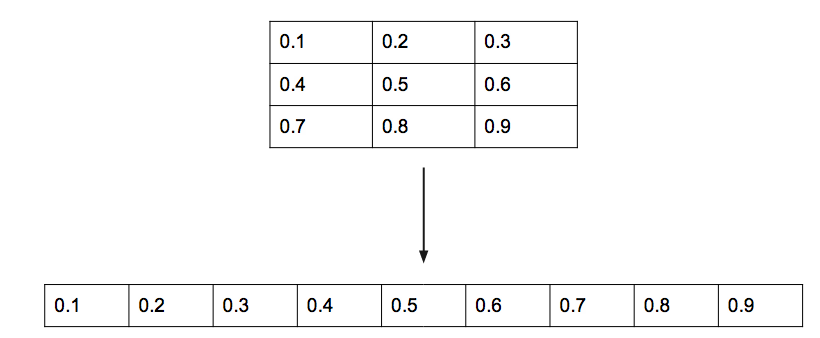
\includegraphics[scale=0.5]{./figures/matrix_to_array.png}
  		\caption{Transformación de la matriz en vector}
  		\label{fig:indiv}
	\end{figure}

\begin{table}[htp]
	\begin{center}
	\begin{tabular}{|c|c|c|c|}
		\hline
	     Fitness & Generación & Corte & $p_{m}$ \\
		\hline
		0.22501570790437642 & 60 & Contenido & 0.05 \\
		0.21842640558999668 & 60 & Contenido & 0.1 \\
		0.22113522454399956 & 67 & Contenido & 0.3 \\ 
		0.22050756611447994 & 72 & Contenido & 0.5 \\
		\hline
	\end{tabular}
	\caption{Configuración simple variando la $p_m$}
	\label{table:simple_mutation_prob}
	\end{center}
\end{table}

\begin{table}[htp]
	\begin{center}
	\begin{tabular}{|c|c|c|c|c|p{1cm}|}
		\hline
	     Fitness & Generación & Corte & $p_{m}$ & decrecimiento (\%) & dec. gen. \\
		\hline
		0.21222349890474348 & 50 & Content & 0.6 & 5 & 30 \\
		0.22795744299992385 & 77 & Content & 0.6 & 10  & 30 \\
		0.21740760693242447 & 65 & Content & 0.6 & 15 & 30 \\
		\hline
	\end{tabular}
	\caption{Configuración simple método de mutación No Uniforme}
	\label{table:simple_mutation_no_uniform}
	\end{center}
\end{table}

\begin{table}[htp]
	\begin{center}
	\begin{tabular}{|c|c|c|c|c|}
		\hline
	     Fitness & Generación & Corte & $p_{m}$ & Cruce \\
		\hline
		0.22501570790437642 & 60 & Contenido & 0.05 & Clásico \\
		0.20662153685787393 & 50 & Contenido & 0.05 & Gene \\
		0.21418198155450324 & 50 & Contenido & 0.05 & Multiples puntos con 2 \\
		0.21674758534799746 & 70 & Contenido & 0.05 & Uniforme con 0.3 prob \\
		0.20662153685787393 & 50 & Contenido & 0.05 & Anular \\
		\hline
	\end{tabular}
	\caption{Configuración simple variando el método de cruce}
	\label{table:crossover}
	\end{center}
\end{table}

\begin{table}[htp]
	\begin{center}
	\begin{tabular}{|c|c|c|c|}
		\hline
	     Nombre .properties & Fitness & Generación & Corte \\
		\hline
		bp\_seb\_rer\_cg\_mc\_ec.properties 		& 16.720276062651436 	& 69 & Contenido \\
		bp\_ser\_reb\_mc\_cc\_emc.properties 	& 11.941655508072634 	& 58 & Contenido \\
		bp\_se\_re\_mc\_cc\_emc.properties 		& 4.825691593990156 	& 51 & Contenido \\
		bp\_seb\_rer\_cmp\_mc\_emc.properties 	& 12.57897997517028 	& 36 & Contenido \\
		bp\_seb\_rer\_mc\_ca\_emc.properties 	& 13.560979676949982 	& 50 & Contenido \\
		bp\_seb\_rer\_mnu\_cc\_emc.properties 	& 12.992838764610976 	& 36 & Contenido \\
		\hline
	\end{tabular}
	\caption{Distintas Configuraciones con backpropagation}
	\label{table:backpropagation}
	\end{center}
\end{table}

\newpage
\begin{lstlisting}[caption={Archivo de configuración simple},label={code:simple}]
popSize = 52
generationGap = 0.6
architecture = 2

mutation = Classic
mutationProbability = 0.05

Backpropagation.probability = 0.15
Backpropagation.iterations = 30

crossover = Classic
crossoverProbability = 1

selection = Elite / Rulette
Elite.toSelect = 16
Rulette.toSelect = 15

replacement = Elite / Boltzman
replacement.Elite.toSelect = 15
replacement.Boltzman.toSelect = 6
replacement.Boltzman.maxTemperature = 100
replacement.Boltzman.minTemperature = 7
replacement.Boltzman.decrement = 0.8


ending = MaxGeneration / Content
MaxGeneration.iterationToEnd = 100
Content.improvement = 0.01
Content.iterationToImprove = 15

\end{lstlisting}


\end{document}
